\chapter{Results}
\label{ch:results}
\section{Comparing algorithms}



\begin{center}
\begin{tabular}{ c c}
 Model              & Accuracy \\
XGBoost            & 83\%     \\
LightGBM           & 82\%     \\
GradientBoosting   & 79\%     \\
LogisticRegression & 76\%   
\end{tabular}
\end{center}
\section{XGBoost}

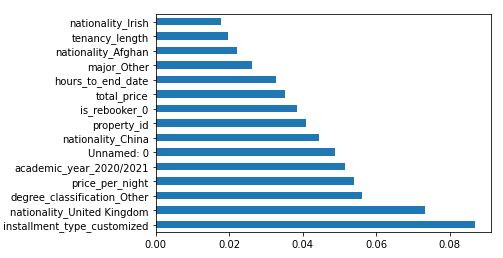
\includegraphics[width=10cm]{figures/results_features.png}

looking at the above figure we can see the feature with most influence on the Target variable is installment type, specifically instalment type customised. This is supported by figure [\textbf{something}] that show students with the instalment type customized are far less likely to cancel. The second most important feature of nationality United Kingdom is likely a dependant feature because the majority of bookings are made by students from the United Kingdom. 
\textbf{i think add a figure to methodology for nationality}
Degree type other being an influencing factor is also supported by figure [\textbf{something}] since students with degree type other where around twice as likely to cancel bookings.




\section{Summary}